\chapter{Teoria tworzenia języków wyskokiego poziomu. }

\section{Gramatyka}
\subsection{Języki formalne}
\defp{Alfabet} lub \defp{słownik} oznaczają dowolny niepusty, skończony zbiór symboli. 
\defp{Słowem} nazywamy ciąg symboli \defp{alfabetu} o skończonej długości.
Jeżeli słowo jest długości zero, to nazywamy go \defp{słowem} pustym,
  które będziemy oznaczać przez małą literę grecką epsilon~($\epsilon$).
  Synonimami \defp{słowa} są \defp{napis} i \defp{zdanie}. \cite{aho}   

  Przykładami \defp{alfabetu} mogą być:
    \begin{itemize}
     \item  zbiór niektórych liter alfabetu polskiego,
     \item  zbiór składający się z symbolu zera i jedynki,
     \item  zbiór liczb całkowitych i zbiór symboli kodowania znaków UTF-8,
     \item  zbiór \{ AA, BB \}, w którym AA i BB są traktowane jako jeden symbol.
    \end{itemize}

  Przykładami  \defp{słów} dla \defp{alfabetu} liczb całkowitych, który składa się ze znaków \{+,-,.(kropka),0,1,2,3,4,5,6,7,8,9\} mogą być:
  $\epsilon$, 0, 1, 01, 10, 090, -1001, +098, -121, 100, +41, +0000010, -000011
itd.
  
Językiem formalnym (językiem) nazywamy podzbiór zbioru wszystkich słów nad skończonym alfabetem.
    
Przykładami języków formalnych mogą być:
\begin{itemize}
 \item zbiór pusty, oznaczany jako \O,
 \item zbiór zawierający tylko słowo puste  \{$\epsilon$\}
 \item zbiór programów, które po skompilowaniu i uruchomieniu zawieszą dany komputer,
 \item zbiór wszystkich poprawnie napisanych nierówności.
\end{itemize}

W tabeli \ref{refoperacje} zostały zdefiniowane prawa na językach.
  
\begin{longtable}{| >{\centering}m{4.5cm}<{\centering} |m{9.5cm}|}
\caption{Definicja operacji na językach.} \label{refoperacje} \\
\hline 
 \multicolumn{1}{|c|}{\textbf{Termin}} & \multicolumn{1}{c|}{\textbf{Definicja}} \\ \hline 
\endfirsthead
\multicolumn{2}{ >{\centering}m{13.5cm}<{\centering}}%
{{ \tablename\ \thetable{} -- Kontynuacja tabeli \mbox{z poprzedniej} strony.}} \\
\hline 
\multicolumn{1}{|c|}{\textbf{Termin}} &
\multicolumn{1}{c|}{\textbf{Definicja}} \\ \hline 
\endhead
%\hline \multicolumn{2}{|r|}{{Kontynuacja na następnej stronie}} \\ \hline
\endfoot
\endlastfoot
        suma $L$ i $M$ zapisywana~$L\bigcup M$ 			& $$L\bigcup M= \{ s : \quad s \in L \quad lub \quad s \in M \}  $$ 	\\ \hline
  	złączenie $L$ i $M$ zapisywane $LM$			& $$ LM = \{ st: \quad s \in L \quad oraz \quad t \in M \} $$  \\ \hline
podnoszenie do potęgi 		    & $$ L^0=\{\epsilon\} $$  $$L^i = L^{i-1}L$$ \\ \hline
domknięcie $L$ zapisywane $L*$ 	& $$ L* = \bigcup_{i=0}^{+\inf} L^i $$	 $L*$  oznacza \cytat{zero lub więcej złączeń} $L$\\ \hline
  dodatnie domknięcie $L$  		zapisywane $L+$  &  $$ L+ = \bigcup_{i=1}^{+\inf} L^i $$	 $L*$  oznacza \cytat{co najmniej jedno złączenie} $L$ \\ \hline
\end{longtable}

	Rozważmy przykład. Niech $L$ będzie zbiorem małych i dużych liter,  a $M$ zbiorem cyfr. Ponieważ symbole mogą być traktowane jako słowa o długości jeden, to zbiory
	$L$ i $M$ są językami skończonymi. Poniżej znajduje się kilka przykładów nowych języków utworzonych za pomocą $L$ i $M$ przy zastosowaniu operatorów zdefiniowanych w~tabeli~\ref{refoperacje}.

\begin{enumerate}
\item $L \bigcup M$  jest zbiorem liter i cyfr.
\item $ML$ jest zbiorem słów składających się z cyfry i występującej po niej litery.
\item $L*$ jest zbiorem wszystkich słów złożonych z liter, włączając w to słowo puste.
\item $L+$ jest zbiorem wszystkich słów złożonych z liter, bez słowa pustego.
\item $L(L \bigcup M )*$ jest zbiorem wszystkich słów złożonych z liter i cyfr, zaczynających się od litery.

\end{enumerate}

\subsection{Gramatyka formalna}
 
Języki formalne opisywane są przez \defp{gramatyki formalne},
to jest uporządkowane czwórki (T,N,P,S), gdzie\cite{aho,link_gramatyka}:
\begin{itemize}
 \item T 
    jest skończonym zbiorem symboli terminalnych (inaczej alfabetem), 
 \item N 
    jest skończonym zbiorem symboli nieterminalnych, przy czym, N$\bigcap$T=\O,
 \item P 
    jest skończonym zbiorem reguł produkcji postaci  $R_1$: $R_2 ;$,
    gdzie $R_1$ i $R_2$,
    to symbole które reprezentują ciągi, o skończonej długości,
    \defp{symboli terminalnych} i \defp{symboli nieterminalnych},
    przy czym, symbol $R_1$ musi zawierać co najmniej jeden symbol nieterminalny.	    
 \item S 
    jest symbolem startowym i należy do zbioru symboli nieterminalnych.
   Od symbolu startowego  zaczyna się wyprowadzanie wszystkich słów danego \defp{języka formalnego}.
\end{itemize}

Rozpatrzmy przykład gramatyki G, która opisuje język akceptujący słowa postaci \{ $(^n)^n: n \in \mathbb{N}$ \},
 Gramatyka G ma postać: 

    G = (  \{ (,) \} , \{S\} , \{S:(S), S: $\epsilon$ \} ,S )
    
Słowo ((())) możemy wyprowadzić:
    S: (S) : ((S)) : (((S))) : ((()))

Do tak opisanego języka należy każde słowo,
 dla którego możliwe jest wyprowadzenie (utworzenie),
 przy użyciu reguł produkcji.
Jeżeli nie jest możliwe wyprowadzenie słowa to nie należy do języka.

\subsection{Klasyfikacja języków} \label{pKlasy}
    
Avram Noam Chomsky badał języki formalne, czyli podzbiór wszystkich słów nad skończonym alfabetem 
wyniku tych badań w 1956r. podał klasyfikację języków formalnych, która powszechnie uznawana jest za standard.


Hierarchia ta składa się z czterech klas \cite{aho, link_eng_chomsky, link_pl_chomsky}:
\begin{itemize}
 \item języki typu 3 - regularne,
   są to języki opisywane za pomocą gramatyki regularnej,
   w której reguły produkcji mogą mieć postać:
      \begin{itemize}
        \item   N:TN
        \item   N:T
        \item   N:N
        \item   N:$\epsilon$
      \end{itemize}
  gdzie N jest symbolem terminalnym, a T symbolem nieterminalnym.

 \item języka typu 2 - bezkontekstowe,
    są to języki opisane za pomocą gramatyk bezkontekstowych,
    w której reguły produkcji mogą mieć postać:
      \begin{itemize}
	\item N:C
      \end{itemize}
    gdzie N jest symbolem nieterminalnym,
    a C to symbole które reprezentują ciągi,
    o skończonej długości,
    symboli terminalnych i symboli nieterminalnych,	  
			   
\item języka typu 1 - kontekstowe,
   opisywany jest przez gramatykę kontekstową, w~której lewa strona produkcji nie może
   zawierać mniej symboli terminalnych i~nieterminalnych niż prawa strona,

\item języka typu 0 - rekurencyjnie przeliczalne,
  opisywany przez gramatykę rekurencyjnie przeliczalną,
  w której reguły produkcji nie zostały ograniczone. 
  
\end{itemize}
 
Mówimy, że język należy do danej klasy wtedy,
 gdy jest możliwe zbudowanie gramatyki,
 która generuje dany język,
 a reguły produkcji nie wykraczają poza ograniczenia dla danej klasy.

\subsection{Wyrażenia regularne}

\defp{Wyrażenie regularne} nad alfabetem $\Sigma$ nazywamy ciąg znaków  $\epsilon$, ), (, *, + oraz symboli z alfabetu $\Sigma$ następującej postaci:

\begin{enumerate}
 \item    $\epsilon$ (słowo puste) jest wyrażeniem regularnym,
 \item wszystkie symbole należące do alfabetu są wyrażeniami regularnymi,
 \item niech $r$ i $s$ będą wyrażeniami regularnymi, to są nimi również:
      \begin{itemize}
       \item $r|s$  (suma),
       \item $rs$   (łączność) ,
       \item $r*$   (domknięcie),
       \item $r+$   (dodatnie domknięcie)
       \item $(r)$  (grupowanie).
      \end{itemize}
 \item wszystkie wyrażenia regularne są postaci opisanej w punkcie 1 -- 3.      
\end{enumerate}

\defp{Wyrażenie regularne} $r$ służy do opisywania języka regularnego,
 który będziemy oznaczać $L(r)$.
Język opisywany przez wyrażenie regularne ma następującą postać:
  \begin{itemize}  
   \item L($\epsilon$) = \{$\epsilon$\}
   \item L($a$) = \{$a$\}, gdzie $a$ jest dowolnym symbolem z alfabetu $\Sigma$
  \end{itemize}
Załóżmy, że $r$ i $s$ jest wyrażeniami regularnymi oznaczającymi języki $L(r)=M$ i $L(s)=L$, wtedy
    \begin{itemize}
     \item $r|s = M\bigcup L$
     \item $rs  = ML$
     \item $r*  = M*$
     \item $r*  = M+$
    \end{itemize}
Operatory na językach zostały opisane w tabeli \ref{refoperacje}, na stronie \pageref{refoperacje}. 
Rozważmy przykłady. Niech alfabet $\Sigma$ będzie zbiór liter języka polskiego oraz cyfr i znaków matematycznych:
  \begin{enumerate}
   \item wyrażenie regularne a$|$b oznacza zbiór \{a,b \},
   \item wyrażenie regularne (a$|$b)* oznacza zbiór \{ $\epsilon$, a, b, aa, ab, bb, ba, aaa, \dots \},
   \item wyrażenie regularne (a$|$b)$|$(a$|$b) oznacza zbiór \{aa,ab,ba,bb\}, 
   \item wyrażenie regularne  $ (-|+) ((1|2|3|4|5|6|7|8|9)(0|1|2|3|4|5|6|7|8|9)*)|0  $ oznacza zbiór wszystkich liczb całkowitych. 	
  \end{enumerate}


\section{Język wysokiego poziomu }

Językiem wysokiego poziomu \ang{High-level language} nazywamy język, 
którego składnia i słowa kluczowe języka ułatwiają użytkownikom  napisanie programu, bądź skrypty,
jak również powinien być on wolny od zależności sprzętowych i systemowych.

Celem niniejszej pracy jest napisanie języka wysokiego poziomu, który będzie językiem interpretowany.
Na rysunku \ref{fig:etapy} został przedstawione etapy budowania, są to:
\begin{enumerate}
 \item Analizator leksykalny  --- czynności związane z analizą leksykalną, które  została przedstawiona w podrozdziale  \ref{p_leksykalna},
 \item Analizator składniowy  --- czynności związane z analizą składniową, które  została przedstawiona w podrozdziale  \ref{p_skladniowa},
 \item Analizator semantyczny --- czynności związane z analizą semantyczną, które  została przedstawiona w podrozdziale \ref{p_semantyczna},
 \item Wykonywanie instrukcji --- Po przekazaniu polecenia jest ono wykonywane, zgodnie z założeniem programisty lub zwracany jest błąd.
\end{enumerate}
Pierwsze trzy etapy budowania oprogramowania są takie samie jak dla kompilatorów i~nazywane tzw. kompilatora.\cite{aho}

 \begin{center}
\begin{figure}[H]
  \begin{center}
    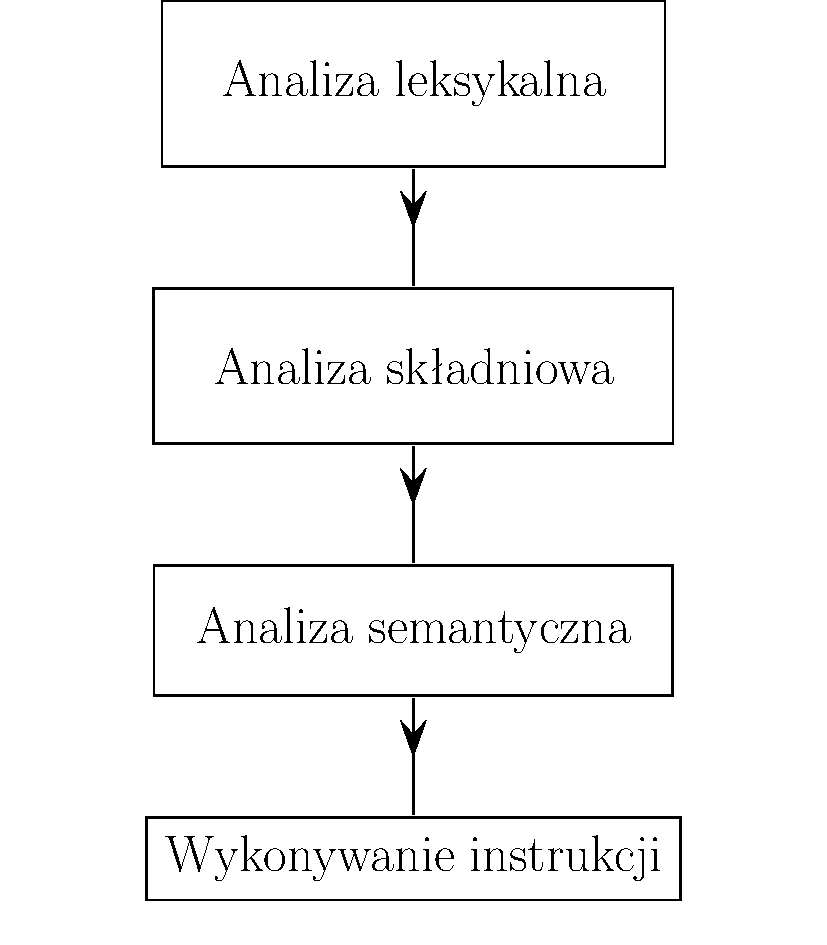
\includegraphics[width=0.7\textwidth, scale=0.5]{etapy.pdf}
  \end{center}
  \caption{Etapy tworzenie języka wysokiego poziomu. }
    \label{fig:etapy}
\end{figure}
\end{center}


\subsection{Analiza leksykalna} \label{p_leksykalna}

Zadaniem analizatora leksykalnego jest tworzenie symboli leksykalnych 
z przesłanego przez użytkownika strumienia znaków na wejście. 
Symbole te są następnie przesyłane  do analizatora składniowego. 
Symbole leksykalne tworzone są na podstawie tablicy wyrażeń regularnych i odpowiadającym i zadaniom,
czyli jeżeli przesłany strumień znaków należy do  n-tego wyrażenie regularne w tabeli 
 to zostanie wykonana powierzone mu zadanie, 
 którym na przykład
 może być \cite{aho}:
\begin{itemize}
 \item Nie wykonanie żadnego działania (strumień znaków zostanie pominięty)
 \item przesłanie symbolu leksykalnego do analizatora
 \item przesłanie symbolu leksykalnego wraz z ciągiem znaków, które należą do wyrażeniami
 \item przesłanie symbolu leksykalnego wraz z modyfikowanym ciągiem znaków
\end{itemize}

Podczas analiz leksykalne możemy zaprojektować analizator leksykalny, 
aby mógł wykrywać następujące błędy:
      \begin{itemize}
	\item   znaki pojawiające się na wejściu nie stanowią żadnego symbolu leksykalnego
	\item   jeśli na wejściu pojawi się znak nie nieobsługiwany 
	\item   gdy istniej możliwość przewidzenia błędnych ciągów znaków odpowiadające jakiemuś symbolowi leksykalnemu.
		Np. operator mniejszy równy \textquotedblleft$>=$\textquotedblright, 
		często jest pisany niepoprawnie w następujący sposób \textquotedblleft$=<$\textquotedblright.
		
		
      \end{itemize}

\subsection{Analiza składniowa} \label{p_skladniowa}


Analizator składniowy otrzymuje od analizatora ciąg symboli leksykalnych,
 które traktowane są jak symbole terminalne w gramatyce. Zadaniem analizatora składniowego,
 jest grupowanie symboli leksykalnych i tworzenie drzewa składniowego zgodnie
 z regułami gramatyki. 
Wynikiem działania analizatora składniowego jest drzewo składniowe lub wyświetlenie komunikatów o błędach.

Drzewem składniowy \ang{parse tree} nazywamy hierarchiczną strukturą danych,
 w której węzły odpowiadają:
\begin{itemize}
  \item  
    symbolu leksykalnemu, czyli skończonemu  ciągowi symboli terminalnych,
  \item  
    symbolu nieterminalnemu.
\end{itemize}


Najpopularniejszymi metodami wykorzystywanymi w analizatorach składniowych
 dla gramatyk są to metody zstępujące i wstępujące.
W metodzie zstępującej drzewo jest tworzone od korzenia do liści,
 a wstępującej odwrotnie od liści do korzenia.
W obu metodach wejście jest przeglądane od lewej strony.

Analizator składniowy może wykryć błędy w przypadku,
 gdy strumień symboli leksykalnych nie jest akceptowany przez gramatykę języka.
Jeżeli zostanie wykryty błąd to analizator składniowy powinien próbować odzyskać kontrolę w celu wykrycia kolejnych błędów
 i~poinformować o nich użytkownika.
Poniżej zostały następujące strategie\cite{aho}:
\begin{description}
  \item[Tryb paniki] --- 
     Po natrafieniu na błąd,
      analizator usuwa symbole leksykalne z wejścia, 
      aż natrafi na symbol z ustalonego zbioru od których może rozpocząć się dalsze poszukiwanie błędów.
  \item[Poziom frazy] --- 
     Pozwala zmienić lub dodać symbole leksykalne,
      które umożliwią dalsze dopasowania,
  \item [Produkcja dla błędu] --- 
     Jeżeli wiemy, 
      gdzie pojawiają się najczęściej błędy,
      to możemy dopisać odpowiednią regułę produkcji w gramatyce.
\end{description}

\subsection{Analiza semantyczna} \label{p_semantyczna}
Kolejnym etapem z rysunku \ref{fig:etapy} na stronie \pageref{fig:etapy} jest analiza semantyczna,
 której zadaniem jest sprawdzenie, 
 czy każdy identyfikator jakiegoś działania nazywany operatorem ma odpowiednią ilość składników nazywane argumentami.
Zadaniem analizatora semantycznego jest również sprawdzenie, czy każdy argument ma odpowiedni typ danych.
Wejściem do analizy semantycznej jest poprawnie zbudowane drzewo składniowe według gramatyk. \cite{aho}

 Błędy semantyczne możemy sklasyfikować w następujący sposób \cite{link_semantic}:
\begin{description}
 \item[Błędy krytyczne] ---
    błędy uniemożliwiające dalszą analizę 
 \item[Błędy tworzące nieoczekiwany] --- 
    istnieją błędy, które nie zostaną przechwycone i zostanie zwrócony nie oczekiwany wynik. Bardzo,
    częstym przykładem tego typu jest program napisany w języku C, który czyta nie ze swojej pamięci,
 \item[Niepotrzebnie rozbudowane polecenia] --- są to polecenia, które zostały podane nadmiarowe dane.
\end{description}


\begin{comment} 
\end{comment}